\section{Langkah-Langkah Percobaan}
A.) Crimping Kabel
\begin{enumerate}
	\item Siapkan perlengkapan berupa Alat Crimping, Tang potong, wire stripper, LAN Tester. Serta bahan-bahan yaitu Kabel UTP dan konektor RJ45
	\item Kupas pelindung luar kabel UTP dengan wire stripper dengan berhati-hati agar tidak melukai kabel yang ada didalam.
	\item pisahkan kabel dengan mengurai kabel yang ada
	\item potong bagian tengah dari kabel yang keras untuk memudahkan proses mengurutkan dan memasukkan kedalam konektor
	\item urutkan kabel yang telah diurai sesuai dengan kode warna. Saat praktikum digunakan protokol T568B, dengan ururtan putih-kuning, kuning, putih-hijau, biru, putih-biru, hijau, putih-coklat, coklat
	\item rapikan ujung kabel, potong bila perlu agar kabel sama panjang, dan luruskan.
	\item masukkan kabel yang telah diurutkan ke konektor RJ45, pastikan ujung kabel sampai kedalam dan tidak tertukar
	\item apabila sudah masuk, gunakan alat crimping untuk mengunci konektor
	\item Uji kabel menggunakan LAN Tester, apabila seluruh lampu menyala secara berurutan maka kabel LAN sudah tercrimping dengan benar.
\end{enumerate}
B.) Routing Statis IPv4
\begin{enumerate}
	\item Reset konfigurasi router
	\item sambungkan laptop dan router menggunakan kabel LAN pada ether1
	\item sambungkan kedua router menggunakan kabel LAN pada ether2
	\item login ke router menggunakan winbox
	\item ubah setting IP ethernet pada laptop menjadi manual, kemudian setting IP Ethernet laptop
	\item tambahkan IP Address router dengan interface Ether1
	\item tambahkan IP Address rotuter lainnya dan gunakan interface Ether2
	\item tambahkan IP Address Laptop lain
	\item uji ping antara laptop dengan router, router dengan router, dan laptop dengan laptop.
\end{enumerate}
C.) Routing Dinamis IPv4
\begin{enumerate}
	\item Reset konfigurasi kedua router, lalu login ke router mikrotik dengan Winbox.
	\item  Aktifkan Routing RIP Package. Konfigurasi IP Address pada Ether1 Tambahkan IP address pada Ether1 yang digunakan sebagai jalur antar-router. 
	\item  Konfigurasi IP Address untuk Jaringan LAN Ether2 Tambahkan IP address pada Ether2 yang digunakan untuk menghubungkan Laptop dengan Router
	\item  Konfigurasi DHCP server dan sesuaikan interface ethernet menjadi 2.
	\item Konfigurasi routing dinamis menggunakan RIP. untuk interface gunakan ether all, setting revice menjadi V1-2, Send menjadi V-2, dan authentification menjadi none
	\item Tambahkan network pada RIP dan masukkan IP network yang ada di router sendiri.
	\item Tambahkan gateway jaringan dengan alamat gateway komputer tujuan.
	\item Konfigurasi IP Adress di Laptop Karena Sekarang sudah menggunakan konfigurasi IP Dinamis maka ubah konfigurasi yang tadi menjadi konfigurasi DHCP
	\item lakukan uji ping
\end{enumerate}

\section{Analisis Hasil Percobaan}
Pada modul 1 praktikum Jaringan Komputer ini dilakukan 3 percobaan. Percobaan pertama adalah tentang crimping kabel. Setelah dilakukan langkah-langkah percobaan praktikan berhasil menyelesaikan percobaan crimping, namun selesai di paling akhir. Ketika melakukan percobaan terdapat kesulitan karena praktikan tidak mengetahui cara melakukan crimping sehingga ketika mengupas pelingdung kabel, bagian dalamnya terluka. Kemudian ketika memasangkan RJ45 ke kabel, bgaian kabel kurang masuk atau kabelnya tertukar sehingga tidak menyala ketika diuji dengan LAN Tester.\\
Pada percobaan kedua, tentang routing statis. Praktikan tidak dapat menyelesaikan percobaan, hanya berhasil melakukan ping antara laptop dengan router. ketika mencoba ping dari laptop ke laptop, di winbox tertulis "unreachable", walau sudah mencoba mengubah-ubah sesuai saran asisten praktikum tetap tidak berhasil. Begitu juga untuk tes ping antar router ke router, setelah diatur kembali untuk interfacenya dan dar winbox telah reachable, namun ketika dilakukan tes ping tetap gagal. Percobaan ketiga, tentang routing dinamis. Praktikan tidak sempat melakukan percobaan ini karena kehabisan waktu.

\section{Hasil Tugas Modul}
\begin{enumerate}
	\item 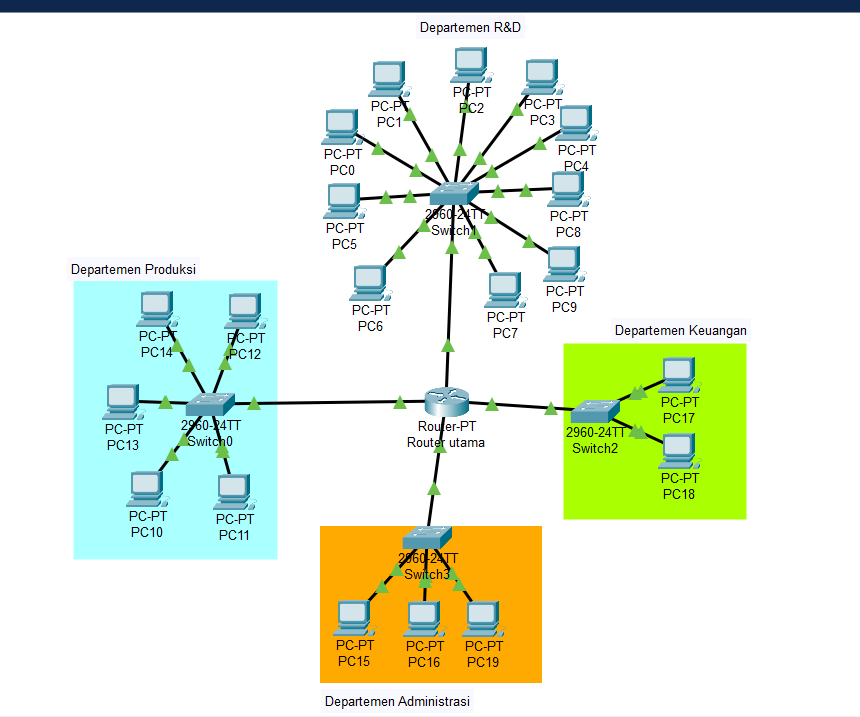
\includegraphics[width=0.8\linewidth,keepaspectratio]{"C:/Users/BINTANG/praktikum-jarkom-main/Laporan Akhir Bintang Narindra/P1/img/Tumod1.png"}\\
	Pada simulasi ini saya menggunakan sejumlah PC untuk mewakili jumlah device yang ada pada setiap departemen. Di setiap departemen PC terhubung antara satu dengan yang lain melalui switch yang juga menguhungkan departemen tersebut dengan Router Utama
	\item Kesulitan saya saat menjalani praktikum adalah saat crimping kabel, ketika mengupas kabel dari pelindung paling luar terlalu dalam, sehingga melukai kabel yang ada didalam selain itu ketika memasangkan konektor kabel tertukar sehingga harus mengulang. Kemudian saat melakukan routing statis, praktikan tidak mengetahui masalah yang terjadi walau sudah mengikuti modul tetap tidak dapat melakukan ping antar router dan ping antar PC
\end{enumerate}

\section{Kesimpulan}
Dari praktikum Jaringan Komputer modul 1 ini didapatkan tentang metode crimping kabel yang benar, dan apa yang harus diperhatikan ketika melakukan crimping seperti saat mengupas pelindung kabel agar tidak melukai kabel yang didalam serta perhatikan kembali urutan kabel setelah memasangkan konektor RJ45 pastikan kembali bahwa urutan tidak tertukar. Untuk routing statis, praktikan memahami secara dasar dari metode routing statis namun tidak mengetahui secara jelas mengapa gagal melakukan ping antar router dan antar pc. Untuk routing dinamis praktikan belum sempat melakukan praktikum karena kehabisan waktu

\section{Lampiran}
\subsection{Dokumentasi saat praktikum}
\begin{figure}[H]
	\centering
	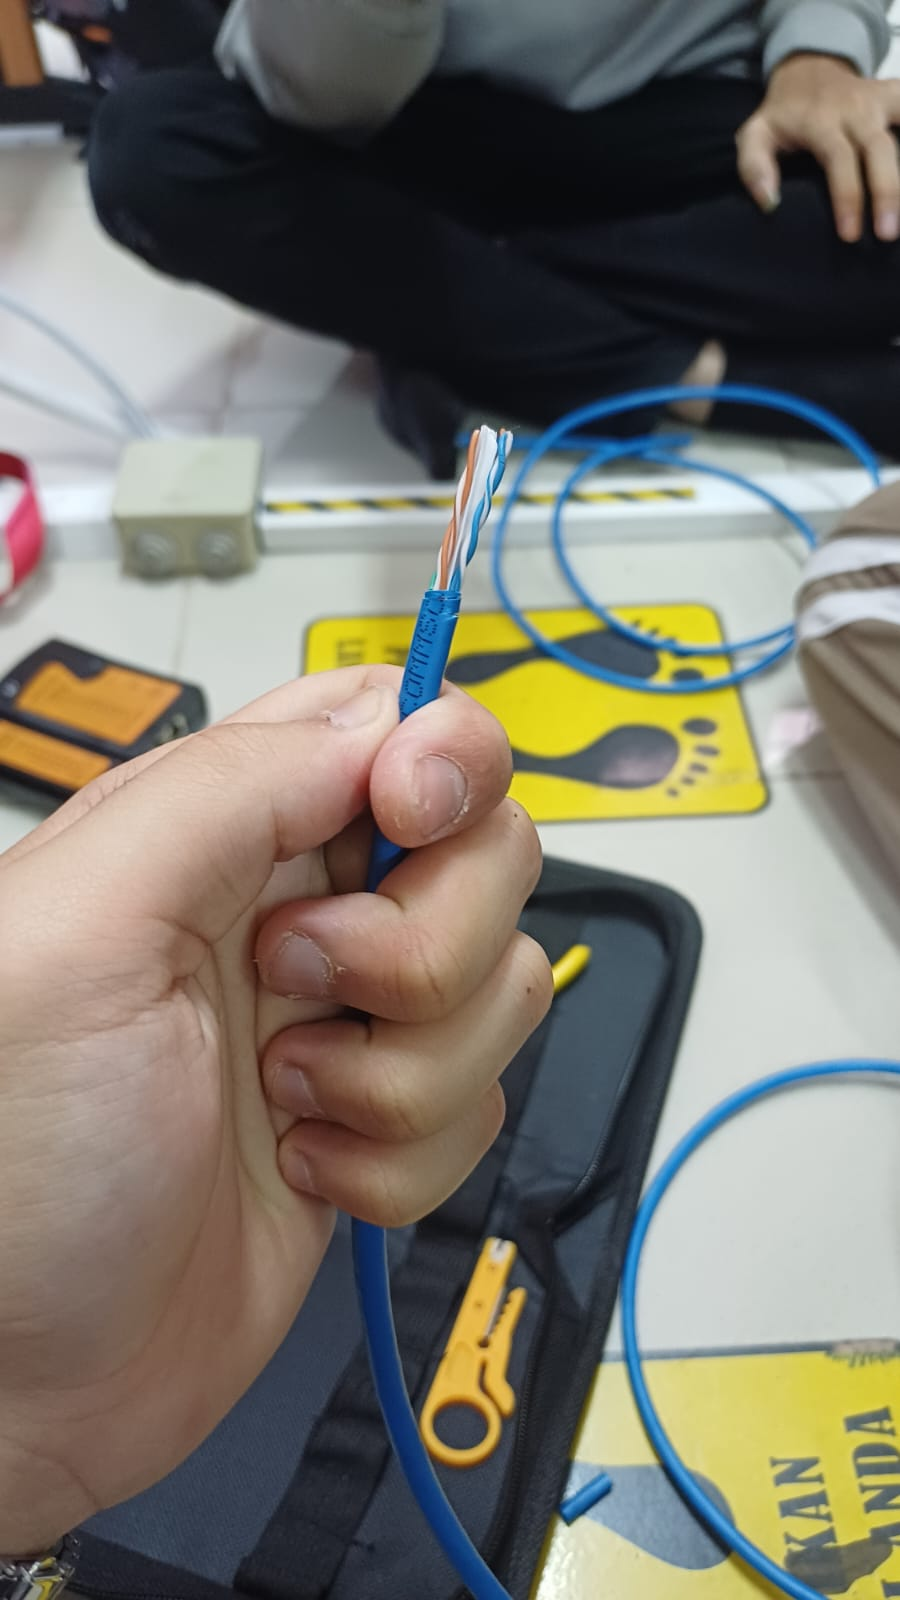
\includegraphics[width=0.3\linewidth,keepaspectratio]{"C:/Users/BINTANG/praktikum-jarkom-main/Laporan Akhir Bintang Narindra/P1/img/crimping1.jpg"}
	\caption{dokumentasi crimping 1}
\end{figure}
\begin{figure}[H]
	\centering
	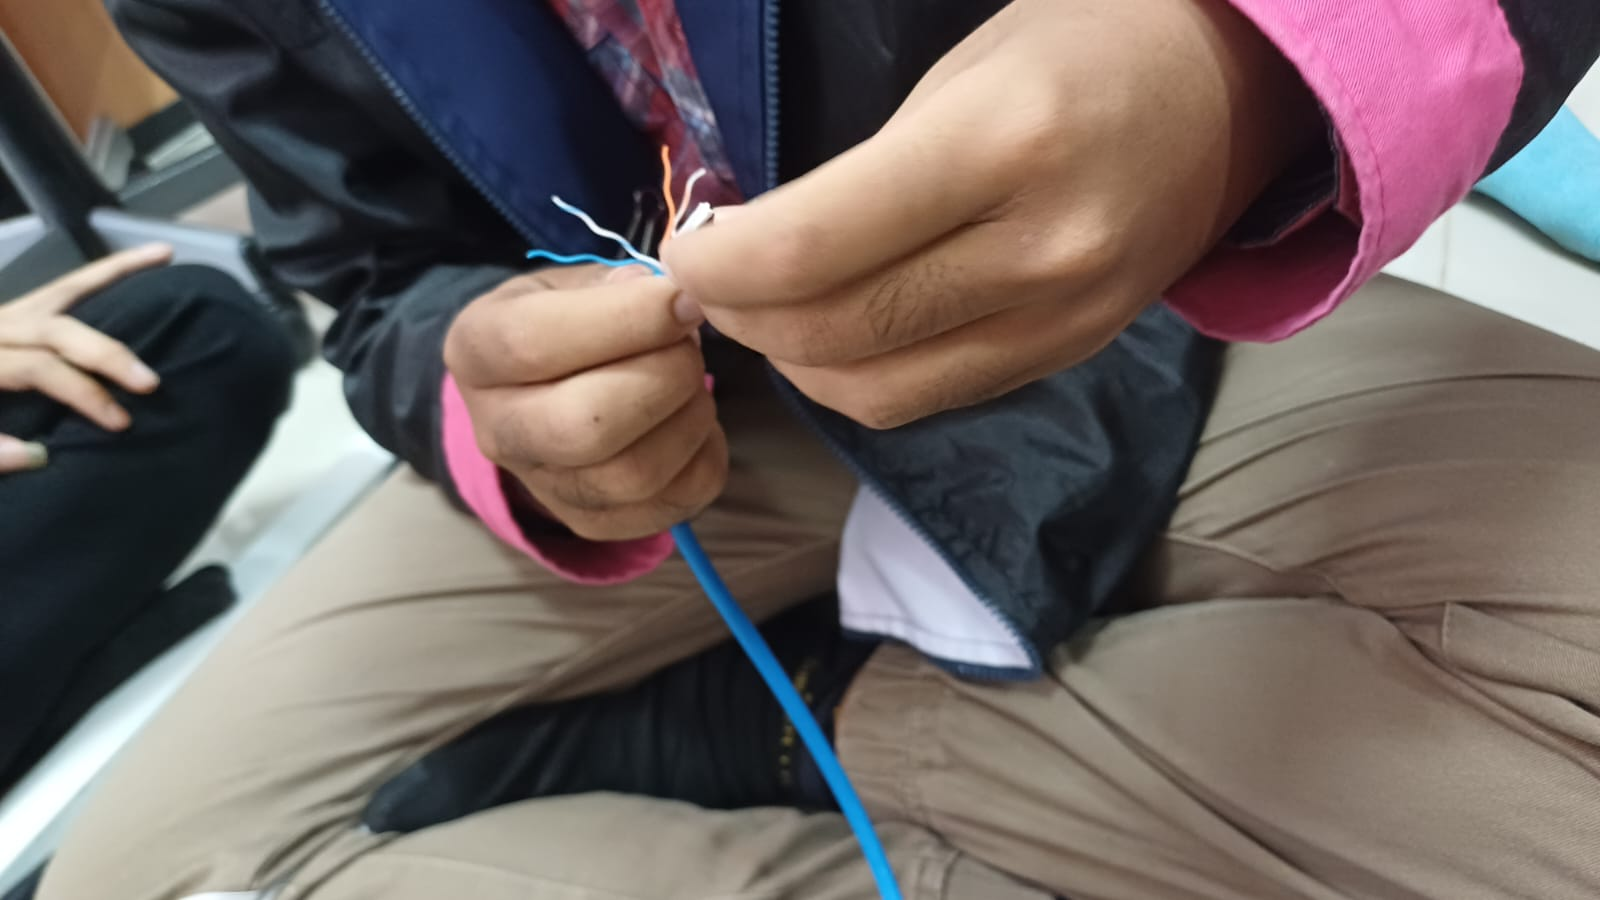
\includegraphics[width=0.5\linewidth,keepaspectratio]{"C:/Users/BINTANG/praktikum-jarkom-main/Laporan Akhir Bintang Narindra/P1/img/crimping2.jpg"}
	\caption{dokumentasi crimping 2}
\end{figure}
\begin{figure}[H]
	\centering
	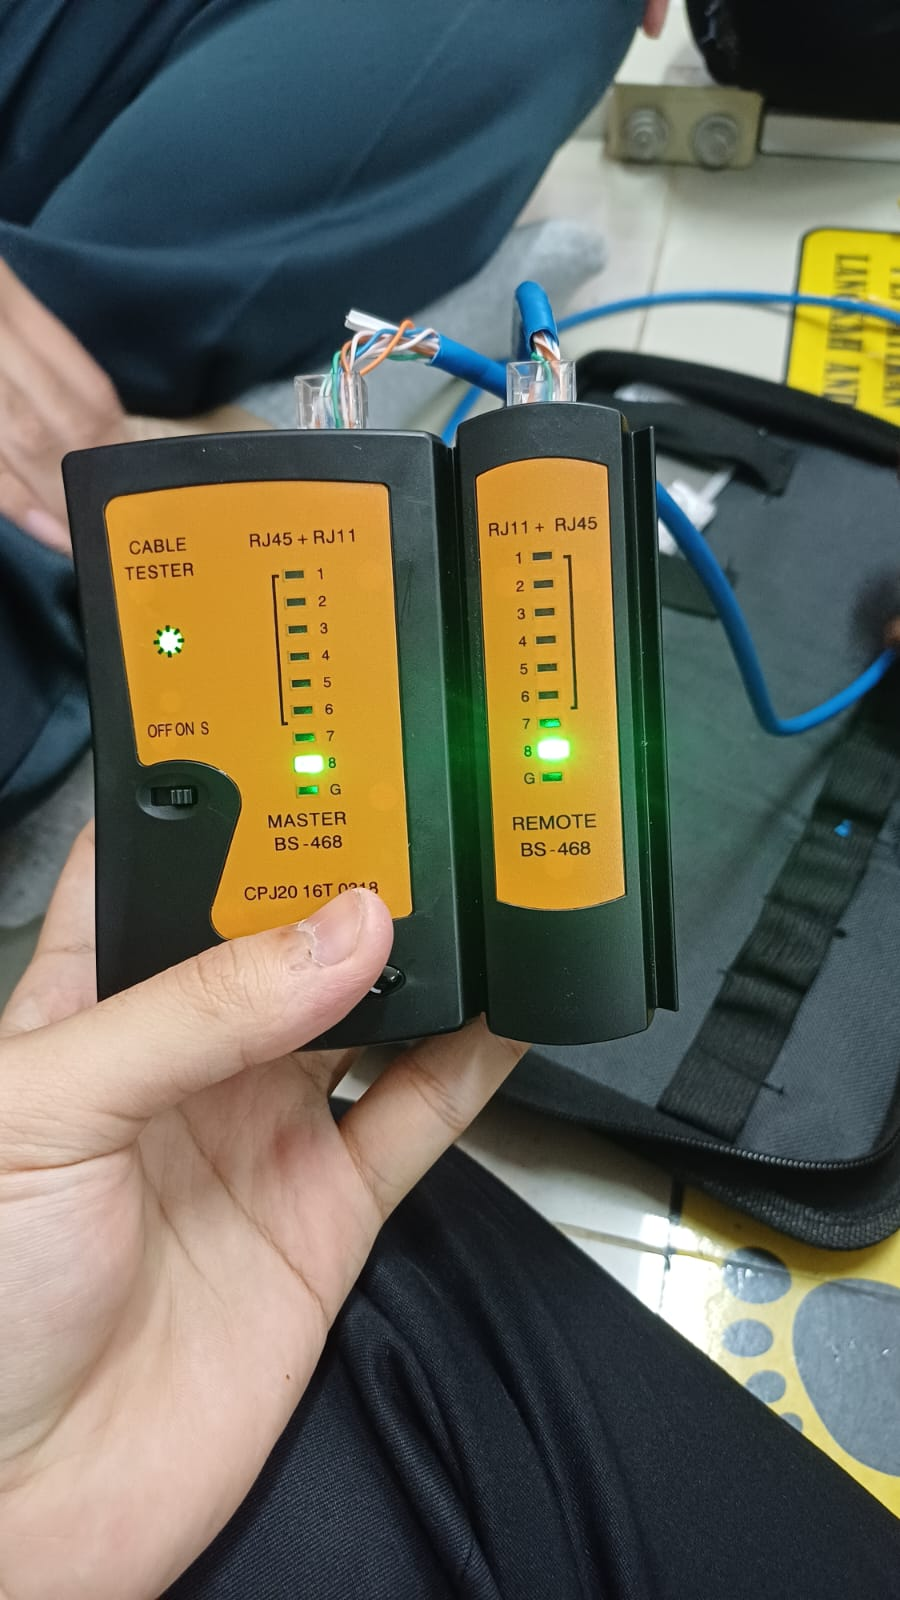
\includegraphics[width=0.3\linewidth,keepaspectratio]{"C:/Users/BINTANG/praktikum-jarkom-main/Laporan Akhir Bintang Narindra/P1/img/hasiltes.jpg"}
	\caption{dokumentasi hasil LAN test}
\end{figure}
\begin{figure}[H]
	\centering
	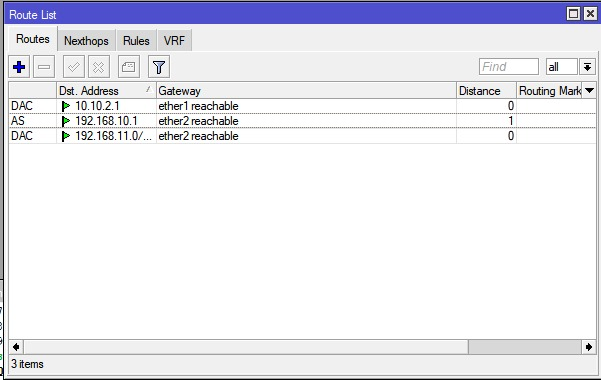
\includegraphics[width=0.5\linewidth,keepaspectratio]{"C:/Users/BINTANG/praktikum-jarkom-main/Laporan Akhir Bintang Narindra/P1/img/setupaddress1.jpg"}
	\caption{dokumentasi address yang di set up}
\end{figure}
\begin{figure}[H]
	\centering
	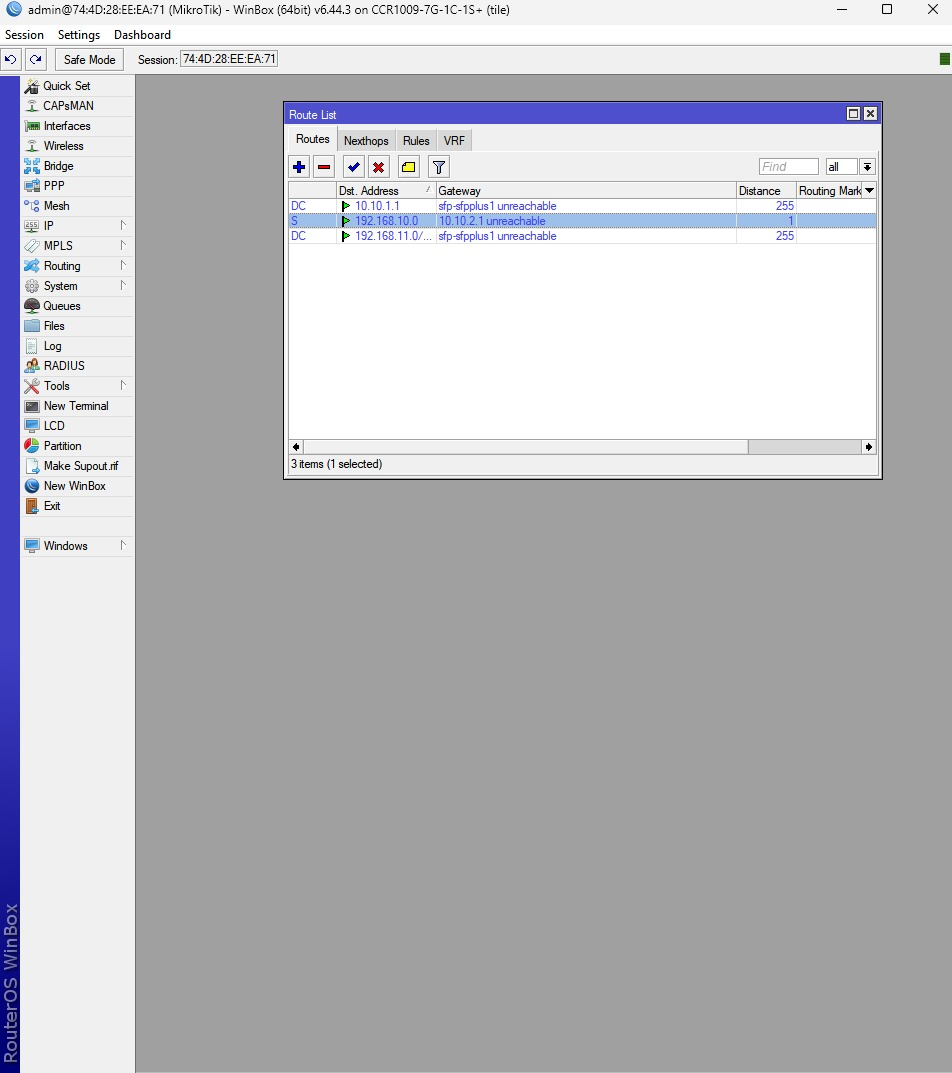
\includegraphics[width=0.3\linewidth,keepaspectratio]{"C:/Users/BINTANG/praktikum-jarkom-main/Laporan Akhir Bintang Narindra/P1/img/route2.jpg"}
	\caption{dokumentasi routing yang diset up}
\end{figure}
\begin{figure}[H]
	\centering
	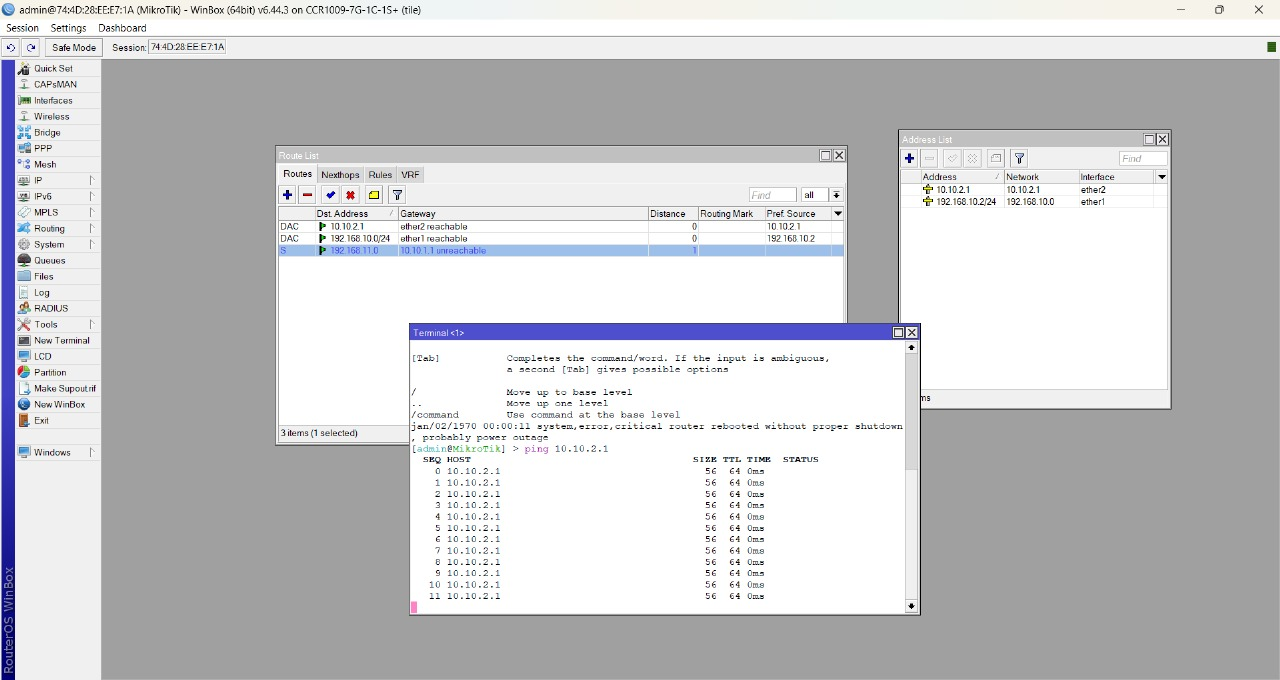
\includegraphics[width=0.5\linewidth,keepaspectratio]{"C:/Users/BINTANG/praktikum-jarkom-main/Laporan Akhir Bintang Narindra/P1/img/tespingrouter2.jpg"}
	\caption{dokumentasi hasil tes ping PC2 dengan router 2}
\end{figure}
\begin{figure}[H]
	\centering
	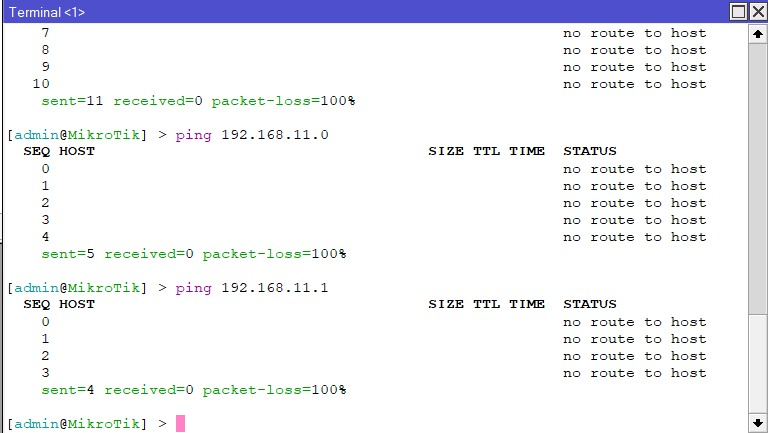
\includegraphics[width=0.5\linewidth,keepaspectratio]{"C:/Users/BINTANG/praktikum-jarkom-main/Laporan Akhir Bintang Narindra/P1/img/pingpcfail.jpg"}
	\caption{dokumentasi hasil tes ping antar PC (gagal)}
\end{figure}
\begin{figure}[H]
	\centering
	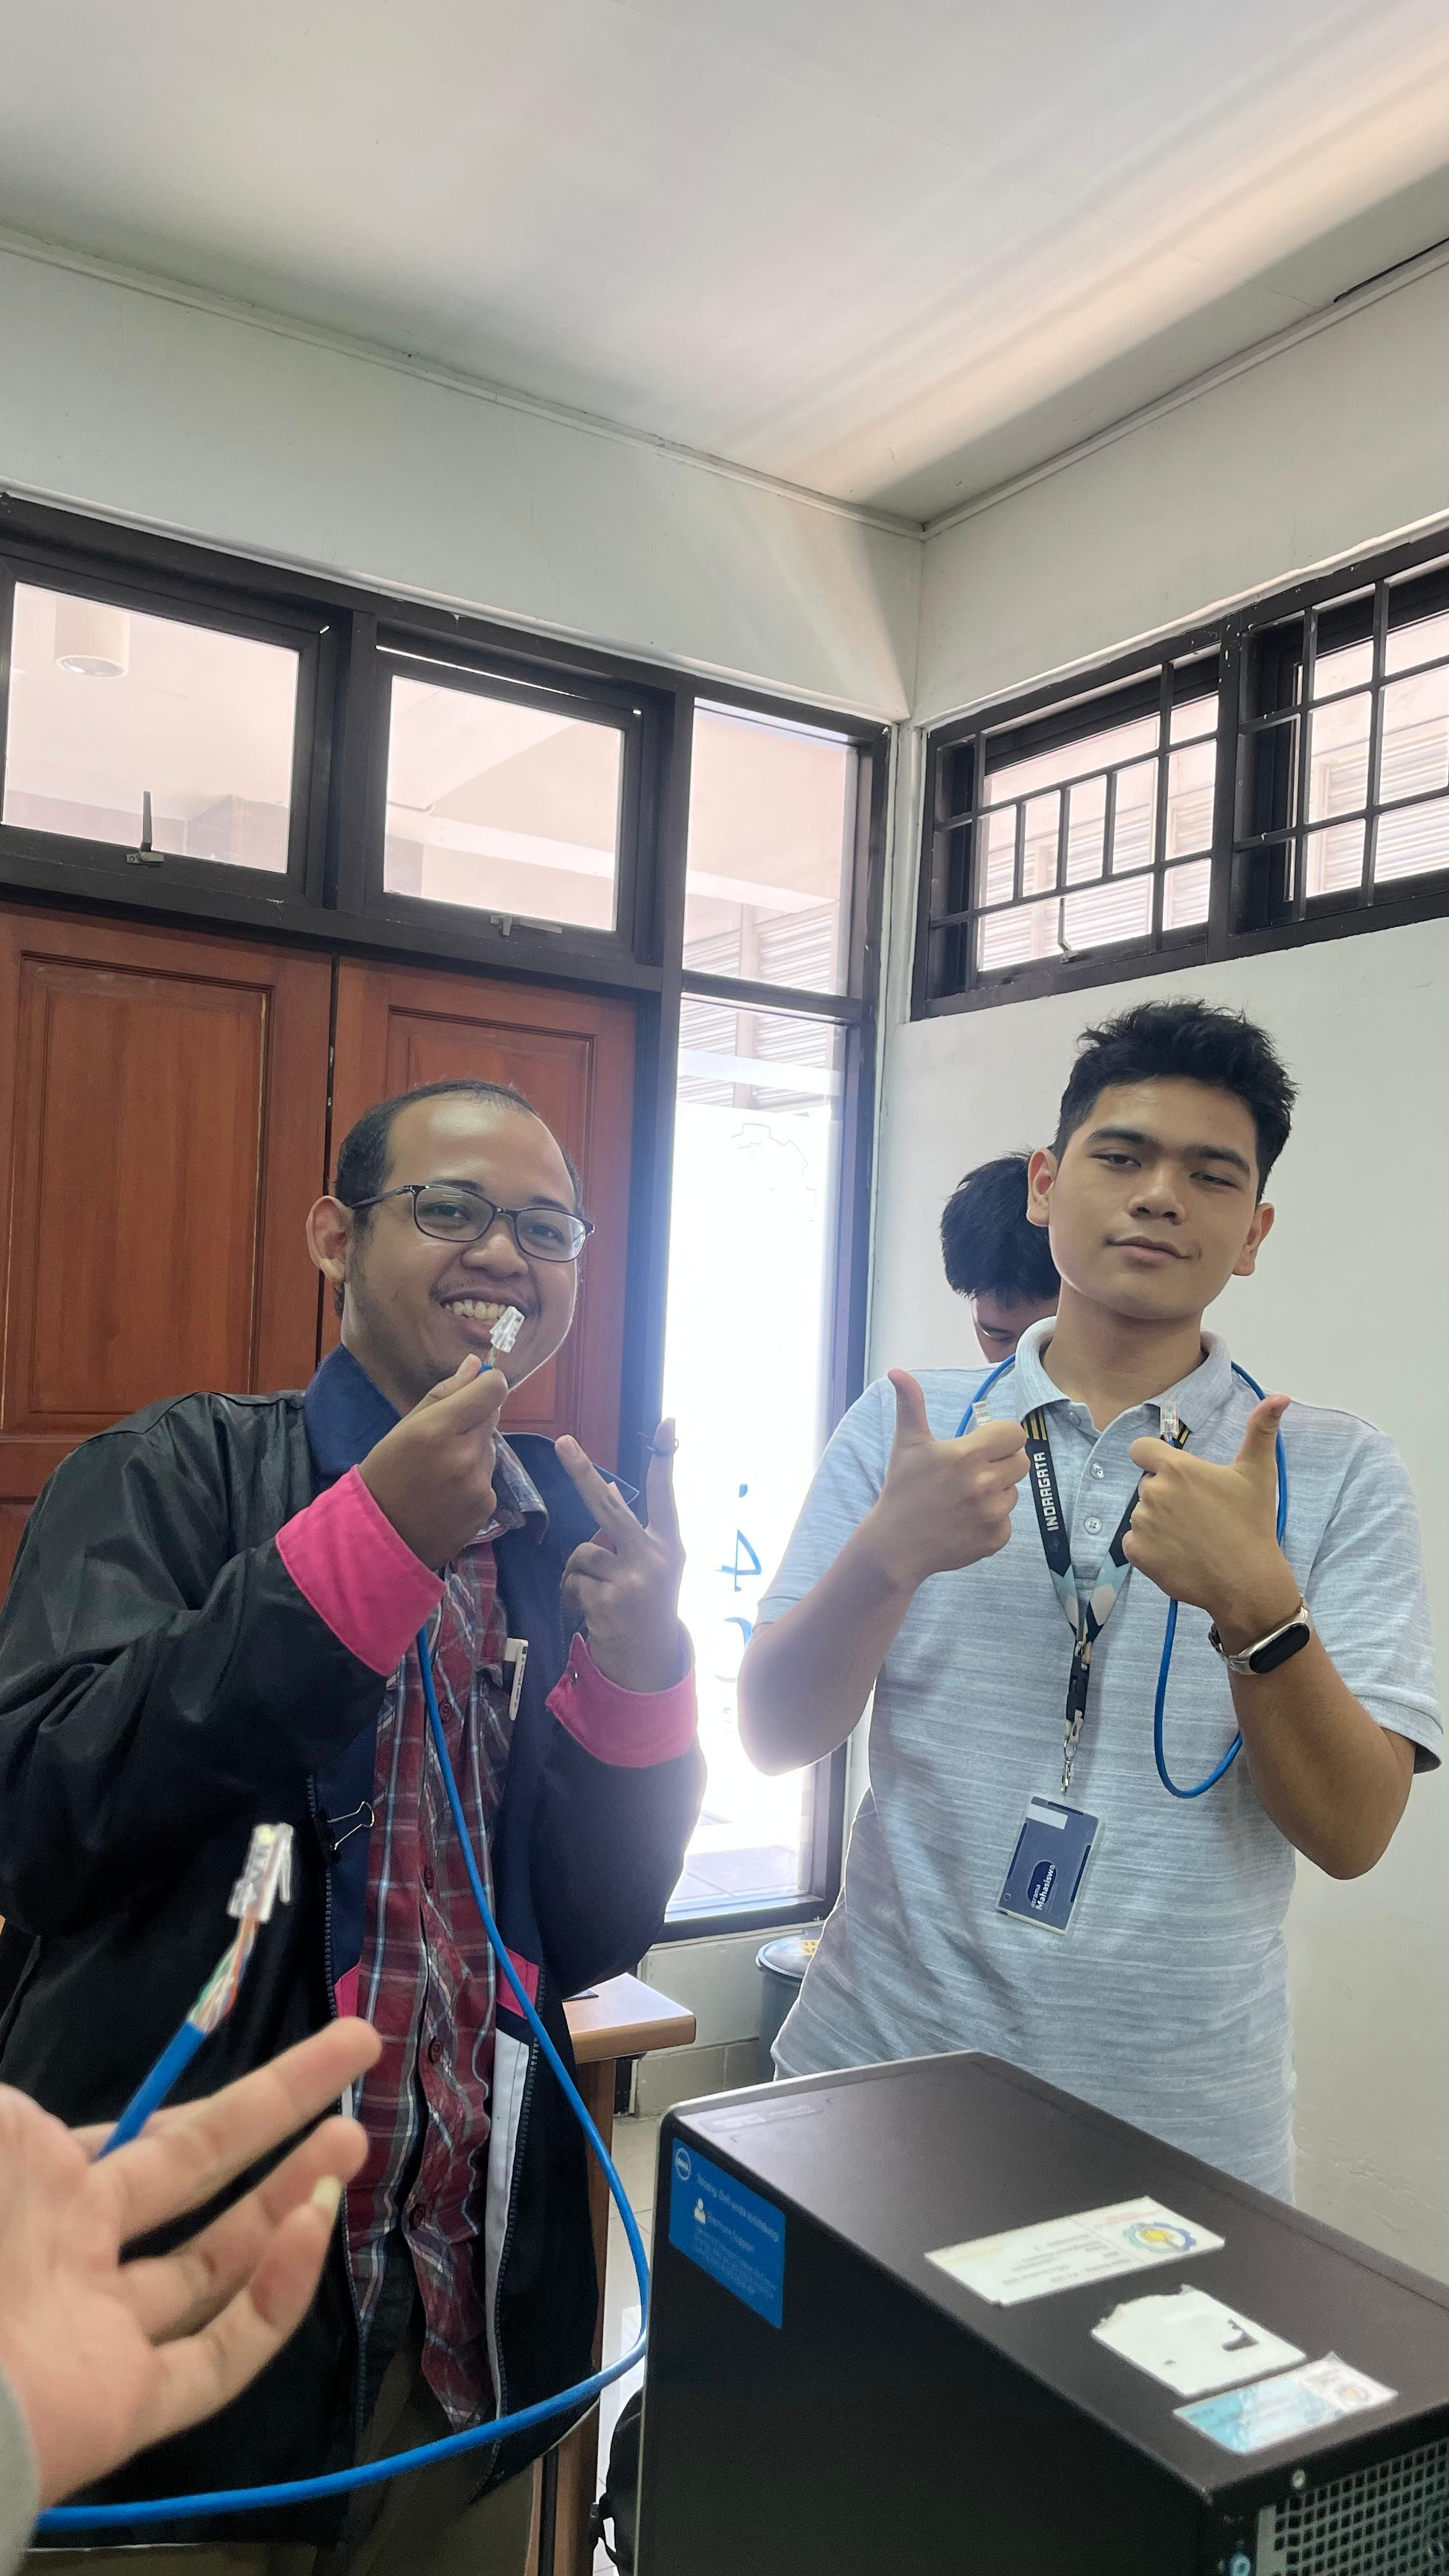
\includegraphics[width=0.3\linewidth,keepaspectratio]{"C:/Users/BINTANG/praktikum-jarkom-main/Laporan Akhir Bintang Narindra/P1/img/pascapraktikum.jpg"}
	\caption{dokumentasi pasca praktikum}
\end{figure}